% ============================================================
%  An Ascon-AEAD128 Hardware Accelerator on an Open RISC-V SoC
%  Ramin Mohammadi Masoudi -- Politecnico di Milano
% ============================================================
\documentclass[aspectratio=169,11pt]{beamer}

\usetheme{default}
\useinnertheme{circles}
\setbeamertemplate{navigation symbols}{}
\setbeamertemplate{itemize items}[circle]

\usepackage[T1]{fontenc}
\usepackage[utf8]{inputenc}
\usepackage{booktabs}
\usepackage{array}
\usepackage{tikz}
\usetikzlibrary{arrows.meta,positioning,calc,fit,backgrounds}
\usepackage{pgfplots}
\pgfplotsset{compat=1.16}
\usepackage{xcolor}
\usepackage{colortbl}

% -- Palette (matched to the written deliverables) -------------
\definecolor{docblue}{RGB}{0,51,102}
\definecolor{doclblue}{RGB}{0,85,128}
\definecolor{okgreen}{RGB}{40,120,70}
\definecolor{warnamber}{RGB}{170,120,0}
\definecolor{hwfill}{RGB}{225,238,252}
\definecolor{swfill}{RGB}{234,245,234}
\definecolor{ratefill}{RGB}{205,228,250}
\definecolor{capfill}{RGB}{238,240,243}
\definecolor{barhw}{RGB}{0,85,128}
\definecolor{barsw}{RGB}{170,120,0}

\setbeamercolor{structure}{fg=docblue}
\setbeamercolor{frametitle}{fg=docblue}
\setbeamercolor{title}{fg=docblue}
\setbeamerfont{frametitle}{series=\bfseries}
\setbeamercolor{block title}{bg=docblue,fg=white}
\setbeamercolor{block body}{bg=docblue!6,fg=black}
\setbeamercolor{alerted text}{fg=warnamber}
\setbeamercolor{section in toc}{fg=docblue}

% -- A quiet, professional footline ---------------------------
\setbeamertemplate{footline}{%
  \hbox{%
  \begin{beamercolorbox}[wd=.5\paperwidth,ht=2.4ex,dp=1.1ex,leftskip=1.2em]{}%
    {\usebeamerfont{date}\color{docblue!70}\scriptsize Ascon-AEAD128 accelerator\ \ $\cdot$\ \ NEORV32\ \ $\cdot$\ \ Tang Nano 20K}%
  \end{beamercolorbox}%
  \begin{beamercolorbox}[wd=.5\paperwidth,ht=2.4ex,dp=1.1ex,rightskip=1.2em]{}%
    \hfill{\usebeamerfont{date}\color{docblue!70}\scriptsize\insertframenumber\,/\,\inserttotalframenumber}%
  \end{beamercolorbox}}%
  \vskip0pt%
}

% -- Section divider with roadmap -----------------------------
\AtBeginSection[]{%
  \begin{frame}[plain]
  \vfill
  \begin{center}
    {\color{docblue}\rule{0.5\textwidth}{0.8pt}}\\[2mm]
    {\Large\bfseries\color{docblue}\insertsectionhead}\\[2mm]
    {\color{docblue}\rule{0.5\textwidth}{0.8pt}}
  \end{center}
  \vspace{3mm}
  \begin{center}
  \begin{minipage}{0.62\textwidth}
  \small
  \tableofcontents[currentsection, sectionstyle=show/shaded, subsectionstyle=hide]
  \end{minipage}
  \end{center}
  \vfill
  \end{frame}
}

\newcommand{\code}[1]{\texttt{\small #1}}
\newcommand{\ok}{\textbf{\color{okgreen}\checkmark}}

\title{\textbf{An Ascon-AEAD128 Hardware Accelerator}}
\subtitle{Model-driven design on a fully open RISC-V SoC, validated on silicon}
\author{Ramin Mohammadi Masoudi}
\institute{Politecnico di Milano}
\date{}

\begin{document}

% ---- Title ----
\begin{frame}[plain]
\titlepage
\vspace{-4mm}
\begin{center}\small\color{docblue}
NEORV32 RISC-V SoC \quad$\cdot$\quad Tang Nano 20K \quad$\cdot$\quad fully-open toolchain
\end{center}
\end{frame}

% ---- Outline ----
\begin{frame}{Outline}
\vspace{2mm}
\begin{columns}[T]
\begin{column}{0.55\textwidth}
\tableofcontents
\end{column}
\begin{column}{0.45\textwidth}
\begin{block}{In one sentence}
\small A hardware accelerator for the NIST lightweight-cryptography standard,
\emph{generated} from a verified model, integrated into an open RISC-V SoC, and
measured on real hardware.
\end{block}
\end{column}
\end{columns}
\end{frame}

% ============================================================
\section{Motivation}

\begin{frame}{Why this project}
\begin{columns}[T]
\begin{column}{0.56\textwidth}
\begin{itemize}
\item \textbf{Ascon} is the NIST standard for lightweight authenticated
      encryption (SP~800-232) --- built for sensors, embedded controllers, IoT
      nodes.
\item Its permutation works on five \textbf{64-bit} words. On a \textbf{32-bit}
      microcontroller every 64-bit rotation costs several instructions.
\item So Ascon in software is slowest exactly on the devices it targets.
      That is the gap hardware should close.
\end{itemize}
\end{column}
\begin{column}{0.44\textwidth}
\begin{block}{Four objectives}
\small
\begin{enumerate}
\item Hardware Ascon that matches the standard, provably
\item A clean C interface on a RISC-V SoC
\item An open, reproducible toolchain
\item Validate on real hardware and \emph{measure}
\end{enumerate}
\end{block}
\end{column}
\end{columns}
\end{frame}

% ============================================================
\section{The algorithm}

\begin{frame}{What authenticated encryption has to provide}
\begin{columns}[T]
\begin{column}{0.55\textwidth}
\small
An AEAD scheme takes a \textbf{key}, a \textbf{nonce}, some \textbf{associated
data} and a \textbf{message}, and must deliver three things at once:
\vspace{2mm}
\begin{enumerate}\small
\item \textbf{Confidentiality} --- the message is unreadable without the key.
\item \textbf{Integrity \& authenticity} --- \emph{any} modification is detected.
      This is the \textbf{tag}: 128 bits that verify or don't.
\item \textbf{Associated data} --- authenticated but \emph{not} encrypted. A packet
      header you must be able to read, but nobody may alter.
\end{enumerate}
\vspace{2mm}
{\small Encryption alone is not enough: without a tag, an attacker can flip bits
in the ciphertext and you would never know.}
\end{column}
\begin{column}{0.45\textwidth}
\centering
\scalebox{0.72}{%
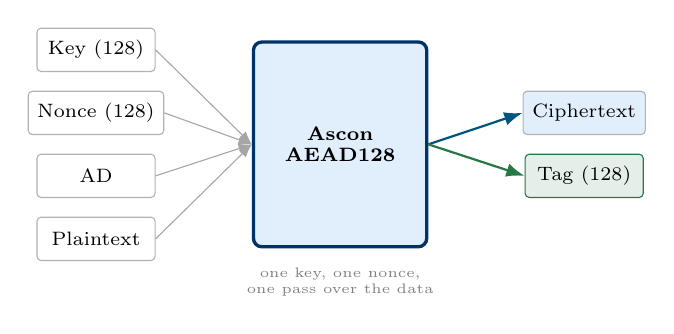
\begin{tikzpicture}[font=\scriptsize, >=Latex,
  io/.style={draw=gray!60, fill=white, rounded corners=1.5pt, minimum width=15mm,
             minimum height=5.5mm},
  eng/.style={draw=docblue, fill=hwfill, very thick, rounded corners=3pt,
              minimum width=22mm, minimum height=26mm}]
\node[io] (k)  at (0,2.4) {Key (128)};
\node[io] (n)  at (0,1.6) {Nonce (128)};
\node[io] (ad) at (0,0.8) {AD};
\node[io] (p)  at (0,0.0) {Plaintext};
\node[eng] (e) at (3.1,1.2) {\shortstack{\textbf{Ascon}\\\textbf{AEAD128}}};
\node[io, fill=hwfill] (c) at (6.2,1.6) {Ciphertext};
\node[io, fill=okgreen!12, draw=okgreen] (t) at (6.2,0.8) {Tag (128)};
\foreach \s in {k,n,ad,p}{\draw[->, gray!70] (\s.east) -- (e.west);}
\draw[->, doclblue, thick] (e.east) -- (c.west);
\draw[->, okgreen, thick] (e.east) -- (t.west);
\node[font=\tiny, gray, align=center] at (3.1,-0.55) {one key, one nonce,\\one pass over the data};
\end{tikzpicture}}
\end{column}
\end{columns}
\end{frame}

\begin{frame}{Ascon is a sponge: one 320-bit state}
\begin{columns}[c]
\begin{column}{0.55\textwidth}
\centering
\scalebox{0.88}{%
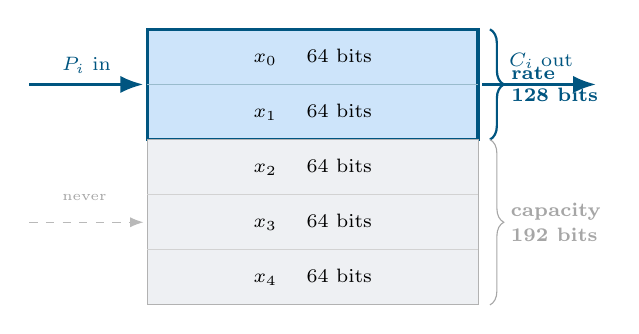
\begin{tikzpicture}[font=\scriptsize, >=Latex]
\draw[draw=doclblue, fill=ratefill, very thick] (0,1.35) rectangle (4.2,2.75);
\node at (2.1,2.4) {$x_0$ \quad 64 bits};
\draw[doclblue!40] (0,2.05) -- (4.2,2.05);
\node at (2.1,1.7) {$x_1$ \quad 64 bits};
\draw[draw=gray!60, fill=capfill] (0,-0.75) rectangle (4.2,1.35);
\node at (2.1,1.0) {$x_2$ \quad 64 bits};
\draw[gray!35] (0,0.65) -- (4.2,0.65);
\node at (2.1,0.3) {$x_3$ \quad 64 bits};
\draw[gray!35] (0,-0.05) -- (4.2,-0.05);
\node at (2.1,-0.4) {$x_4$ \quad 64 bits};
\draw[decorate, decoration={brace, amplitude=5pt}, doclblue, thick]
  (4.35,2.75) -- (4.35,1.35) node[midway, right=4pt, doclblue, font=\scriptsize\bfseries]
  {\shortstack[l]{\textbf{rate}\\128 bits}};
\draw[decorate, decoration={brace, amplitude=5pt}, gray!70]
  (4.35,1.35) -- (4.35,-0.75) node[midway, right=4pt, gray!70, font=\scriptsize\bfseries]
  {\shortstack[l]{\textbf{capacity}\\192 bits}};
\draw[->, doclblue, very thick] (-1.5,2.05) -- (-0.05,2.05)
  node[midway, above, font=\scriptsize, doclblue] {$P_i$ in};
\draw[->, doclblue, very thick] (4.25,2.05) -- (5.7,2.05);
\node[font=\scriptsize, doclblue] at (5.0,2.35) {$C_i$ out};
\draw[->, gray!55, dashed] (-1.5,0.3) -- (-0.05,0.3);
\node[font=\tiny, gray!70] at (-0.8,0.62) {never};
\end{tikzpicture}}
\end{column}
\begin{column}{0.45\textwidth}
\small
\begin{itemize}
\item \textbf{320 bits}: five 64-bit words.
\item Data \textbf{only touches the rate} --- the top 128 bits. XOR a block in; the
      rate becomes the ciphertext.
\item The \textbf{capacity} is never read or written by data. It carries the
      security.
\item Between blocks the permutation stirs all 320 bits.
\end{itemize}
\vspace{1mm}
{\small\color{docblue}\textbf{Why this matters for hardware}}\\
{\small Encryption, hashing and XOF share the \emph{same} state and \emph{same}
permutation --- only the IV and padding differ. \textbf{One permutation is the
entire engine.}}
\end{column}
\end{columns}
\end{frame}

\begin{frame}{Ascon-AEAD128: four phases}
\centering
\scalebox{0.95}{%
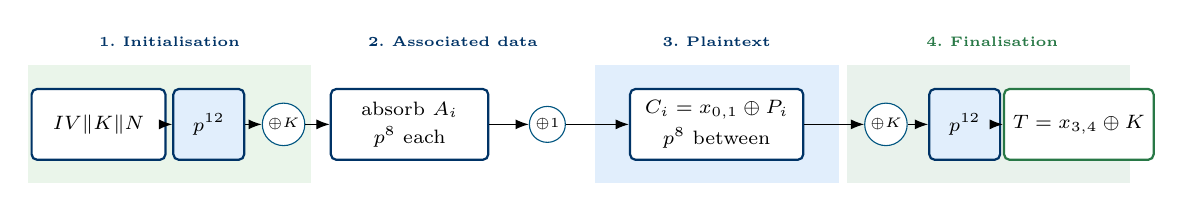
\begin{tikzpicture}[font=\scriptsize, >=Latex,
  s/.style={draw=docblue, thick, rounded corners=2pt, align=center,
            minimum height=9mm, inner sep=3pt},
  p/.style={s, fill=hwfill, minimum width=9mm},
  xo/.style={circle, draw=doclblue, fill=white, inner sep=1.2pt, font=\tiny}]

% --- phase bands (drawn first, behind) ---
\fill[swfill]      (-0.55,-0.75) rectangle (3.05,0.75);
\fill[white]       (3.15,-0.75)  rectangle (6.55,0.75);
\fill[hwfill]      (6.65,-0.75)  rectangle (9.75,0.75);
\fill[okgreen!10]  (9.85,-0.75)  rectangle (13.45,0.75);
\foreach \x/\lbl/\col in {1.25/{1.\ Initialisation}/docblue, 4.85/{2.\ Associated data}/docblue,
                          8.2/{3.\ Plaintext}/docblue, 11.7/{4.\ Finalisation}/okgreen}{
  \node[font=\tiny\bfseries, \col] at (\x,1.05) {\lbl};
}

% --- the chain ---
\node[s, fill=white, minimum width=17mm] (iv) at (0.35,0) {$IV \Vert K \Vert N$};
\node[p] (p12a) at (1.75,0) {$p^{12}$};
\node[xo] (k1) at (2.7,0) {$\oplus K$};
\node[s, fill=white, minimum width=20mm] (ad) at (4.3,0) {\shortstack{absorb $A_i$\\$p^{8}$ each}};
\node[xo] (ds) at (6.05,0) {$\oplus 1$};
\node[s, fill=white, minimum width=22mm] (pt) at (8.2,0) {\shortstack{$C_i = x_{0,1}\oplus P_i$\\$p^{8}$ between}};
\node[xo] (k2) at (10.35,0) {$\oplus K$};
\node[p] (p12b) at (11.35,0) {$p^{12}$};
\node[s, minimum width=19mm, fill=white, draw=okgreen] (tag) at (12.8,0) {$T = x_{3,4}\oplus K$};

\draw[->](iv)--(p12a); \draw[->](p12a)--(k1); \draw[->](k1)--(ad);
\draw[->](ad)--(ds); \draw[->](ds)--(pt); \draw[->](pt)--(k2);
\draw[->](k2)--(p12b); \draw[->](p12b)--(tag);
\end{tikzpicture}}

\vspace{7mm}
\begin{columns}[T]
\begin{column}{0.48\textwidth}
\begin{block}{Parameters, from the standard}
\small
\code{IV = 0x00001000808c0001}\\[1mm]
rate \textbf{16 bytes} \quad $a = 12$ \quad $b = 8$ \quad tag \textbf{128 bits}
\end{block}
\end{column}
\begin{column}{0.52\textwidth}
\small
\textbf{Associated data} is authenticated but \emph{not} encrypted --- a header you
must not tamper with, but need to read in clear.\\[1.5mm]
The \textbf{tag} is what makes this \emph{authenticated} encryption: flip one bit
of the ciphertext and it stops verifying. \alert{I will show that on the board.}
\end{column}
\end{columns}
\end{frame}

\begin{frame}{Phases 1 \& 2: initialisation, associated data}
\begin{columns}[T]
\begin{column}{0.54\textwidth}
\textbf{1. Initialisation}
\begin{itemize}\small
\item Load directly: $x_0 \leftarrow IV$, \ $x_1\Vert x_2 \leftarrow K$, \
      $x_3\Vert x_4 \leftarrow N$.
\item Run $p^{12}$, then XOR the key in \emph{again}:
      $x_3 \mathrel{\oplus}= K_0$, $x_4 \mathrel{\oplus}= K_1$.
\end{itemize}
{\footnotesize\alert{Why twice?} The key enters before \emph{and} after a full
12-round permutation --- so the state depends on it in a way an attacker cannot
unwind.}
\vspace{2mm}

\textbf{2. Associated data}
\begin{itemize}\small
\item Per 16-byte block: $x_0\Vert x_1 \mathrel{\oplus}= A_i$, then $p^{8}$.
\item Padding: append \code{0x01}, then zeros --- and if the AD is already a
      multiple of the rate, absorb an \textbf{extra all-padding block}.
\item \textbf{Domain separation}: $x_4 \mathrel{\oplus}= 1\!\ll\!63$ --- the last
      bit of the 320-bit state.
\end{itemize}
\end{column}
\begin{column}{0.46\textwidth}
\vspace{1mm}
\centering
\scalebox{0.82}{%
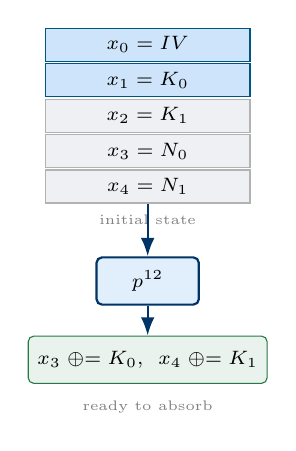
\begin{tikzpicture}[font=\scriptsize, >=Latex,
  st/.style={draw=doclblue, fill=ratefill, minimum width=26mm, minimum height=4.2mm, inner sep=1pt},
  cp/.style={draw=gray!60, fill=capfill, minimum width=26mm, minimum height=4.2mm, inner sep=1pt}]
\node[st] (a0) at (0,2.2) {$x_0 = IV$};
\node[st] (a1) at (0,1.75) {$x_1 = K_0$};
\node[cp] (a2) at (0,1.3) {$x_2 = K_1$};
\node[cp] (a3) at (0,0.85) {$x_3 = N_0$};
\node[cp] (a4) at (0,0.4) {$x_4 = N_1$};
\node[font=\tiny, gray] at (0,-0.02) {initial state};
\node[draw=docblue, fill=hwfill, thick, rounded corners=2pt,
      minimum width=13mm, minimum height=6mm] (p12) at (0,-0.8) {$p^{12}$};
\draw[->, docblue, thick] (0,0.18) -- (p12.north);
\node[draw=okgreen, fill=okgreen!10, rounded corners=2pt,
      minimum width=30mm, minimum height=6mm, font=\scriptsize] (kx) at (0,-1.8)
      {$x_3 \mathrel{\oplus}= K_0$, \ $x_4 \mathrel{\oplus}= K_1$};
\draw[->, docblue, thick] (p12.south) -- (kx.north);
\node[font=\tiny, gray] at (0,-2.4) {ready to absorb};
\end{tikzpicture}}
\end{column}
\end{columns}
\end{frame}

\begin{frame}{Phases 3 \& 4: plaintext, finalisation}
\begin{columns}[T]
\begin{column}{0.54\textwidth}
\textbf{3. Plaintext}
\begin{itemize}\small
\item XOR the block into the rate --- and the rate \emph{becomes} the ciphertext:
      $C_i = (x_0\Vert x_1) \oplus P_i$.
\item Then $p^{8}$ \emph{between} blocks --- but \textbf{not} after the last;
      finalisation follows immediately.
\end{itemize}
{\footnotesize\alert{The elegance:} absorbing the plaintext and producing the
ciphertext are \emph{the same XOR}. Decryption differs only in which value you
keep.}
\vspace{2mm}

\textbf{4. Finalisation}
\begin{itemize}\small
\item $x_2 \mathrel{\oplus}= K_0$, \ $x_3 \mathrel{\oplus}= K_1$, then $p^{12}$.
\item Tag: $T = (x_3 \oplus K_0)\Vert(x_4 \oplus K_1)$.
\end{itemize}
{\footnotesize The tag depends on the key, the nonce, \emph{every} AD byte and
\emph{every} message byte. Change one and it fails.}
\end{column}
\begin{column}{0.46\textwidth}
\vspace{2mm}
\centering
\scalebox{0.85}{%
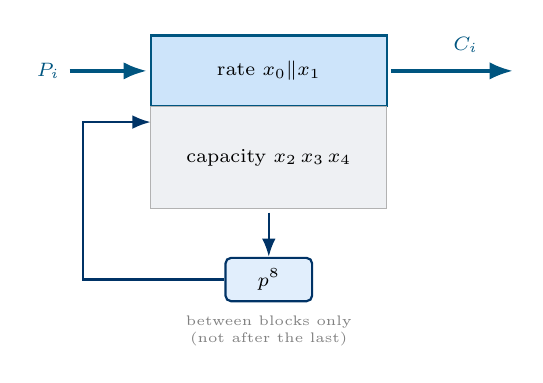
\begin{tikzpicture}[font=\scriptsize, >=Latex]
\draw[draw=doclblue, fill=ratefill, thick] (0,1.5) rectangle (3.0,2.4);
\node at (1.5,1.95) {rate $x_0\Vert x_1$};
\draw[draw=gray!60, fill=capfill] (0,0.2) rectangle (3.0,1.5);
\node at (1.5,0.85) {capacity $x_2\,x_3\,x_4$};
\node[font=\scriptsize, doclblue] (pi) at (-1.3,1.95) {$P_i$};
\draw[->, doclblue, very thick] (pi.east) -- (-0.05,1.95);
\draw[->, doclblue, very thick] (3.05,1.95) -- (4.6,1.95);
\node[font=\scriptsize, doclblue] at (4.0,2.28) {$C_i$};
\node[draw=docblue, fill=hwfill, thick, rounded corners=2pt,
      minimum width=11mm, minimum height=5.5mm] (p8) at (1.5,-0.7) {$p^{8}$};
\draw[->, docblue, thick] (1.5,0.15) -- (p8.north);
\draw[->, docblue, thick] (p8.west) -- ++(-1.8,0) |- (0,1.3);
\node[font=\tiny, gray, align=center] at (1.5,-1.35) {between blocks only\\(not after the last)};
\end{tikzpicture}}
\end{column}
\end{columns}
\end{frame}

\begin{frame}{Inside the permutation: three steps, twelve times}
\begin{columns}[T]
\begin{column}{0.52\textwidth}
\small
\textbf{1. Add round constant} \hfill $p_C$
\begin{itemize}\footnotesize
\item $x_2 \mathrel{\oplus}= c_r$ --- a different constant each round.
\item Breaks the symmetry between rounds.
\end{itemize}
\textbf{2. Substitution} \hfill $p_S$
\begin{itemize}\footnotesize
\item A \textbf{5-bit S-box} --- the \emph{only} non-linear step in the cipher.
\item Applied to a \textbf{bit-column}: one bit from each of $x_0 \ldots x_4$.
\item \textbf{64 columns}, completely \textbf{independent} of one another.
\end{itemize}
\textbf{3. Linear diffusion} \hfill $p_L$
\begin{itemize}\footnotesize
\item Each word XORed with two rotations of itself --- spreading each column's
      result across the word, so next round the columns all differ.
\end{itemize}
\end{column}
\begin{column}{0.48\textwidth}
\vspace{-3mm}
\centering
\scalebox{0.58}{%
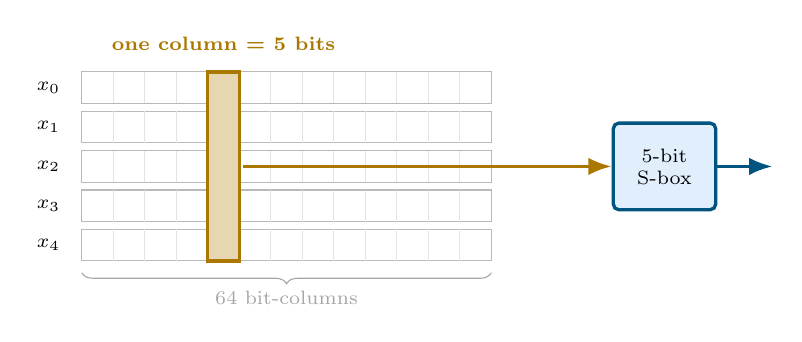
\begin{tikzpicture}[font=\tiny, >=Latex]
\foreach \y/\n in {2.0/$x_0$, 1.5/$x_1$, 1.0/$x_2$, 0.5/$x_3$, 0.0/$x_4$}{
  \node[left, font=\scriptsize] at (-0.15,\y) {\n};
  \draw[draw=gray!55, fill=white] (0,\y-0.2) rectangle (5.2,\y+0.2);
  \foreach \c in {1,...,12}{ \draw[gray!22] (0.4*\c,\y-0.2) -- (0.4*\c,\y+0.2); }
}
\fill[warnamber!30] (1.6,-0.2) rectangle (2.0,2.2);
\draw[warnamber, very thick] (1.6,-0.2) rectangle (2.0,2.2);
\node[warnamber, font=\scriptsize\bfseries, above] at (1.8,2.35) {one column = 5 bits};
\node[draw=doclblue, fill=hwfill, very thick, rounded corners=2pt,
      minimum width=13mm, minimum height=11mm, font=\scriptsize, align=center] (sb) at (7.4,1.0)
      {5-bit\\S-box};
\draw[->, warnamber, very thick] (2.05,1.0) -- (sb.west);
\draw[->, doclblue, very thick] (sb.east) -- ++(0.7,0);
\draw[decorate, decoration={brace, amplitude=4pt, mirror}, gray!70]
  (0,-0.35) -- (5.2,-0.35) node[midway, below=3pt, font=\scriptsize, gray!70] {64 bit-columns};
\end{tikzpicture}}

\vspace{1mm}
{\footnotesize The $p_L$ rotation constants, from the standard:}
{\scriptsize
\[\begin{aligned}[t]
x_0 &\mathrel{\oplus}= (x_0\!\ggg\!19)\oplus(x_0\!\ggg\!28)\\[-0.8mm]
x_1 &\mathrel{\oplus}= (x_1\!\ggg\!61)\oplus(x_1\!\ggg\!39)\\[-0.8mm]
x_2 &\mathrel{\oplus}= (x_2\!\ggg\!1)\ \oplus(x_2\!\ggg\!6)\\[-0.8mm]
x_3 &\mathrel{\oplus}= (x_3\!\ggg\!10)\oplus(x_3\!\ggg\!17)\\[-0.8mm]
x_4 &\mathrel{\oplus}= (x_4\!\ggg\!7)\ \oplus(x_4\!\ggg\!41)
\end{aligned}\]}
\end{column}
\end{columns}
\end{frame}

\begin{frame}{The design lever: one choice spans the whole space}
{\small The 64 S-boxes are \textbf{independent}. Build all 64 and do a round per
cycle --- or build \emph{one} and take 64 cycles per round. That single choice
trades area against time, and spans the entire architecture space.}
\vspace{0.5mm}
\begin{center}
{\scriptsize\setlength{\tabcolsep}{5pt}\renewcommand{\arraystretch}{1.02}
\begin{tabular}{llrl}
\toprule
\textbf{Architecture} & \textbf{S-boxes / cycle} & \textbf{Cycles / $p^{12}$} & \textbf{Natural target}\\
\midrule
bit-serial              & fraction of one & 1\,561 & smallest possible ASIC\\
column-serial, 1 col    & 1               & 793   & minimum-area ASIC\\
column-serial, 8 cols   & 8               & 121   & small ASIC\\
\rowcolor{hwfill}
\textbf{1 round / cycle}& \textbf{64}     & \textbf{13} & \textbf{this board}\\
2 rounds / cycle        & 128             & 7     & FPGA, more area\\
4 rounds / cycle        & 256             & 4     & FPGA, throughput\\
8 rounds / cycle        & 512             & 3     & large FPGA\\
fully pipelined         & 768 (12 stages) & 1\,$^{*}$ & maximum throughput\\
\bottomrule
\end{tabular}}
\end{center}
\vspace{0.5mm}
{\scriptsize $^{*}$ one result per cycle once the 12-stage pipeline is full.
All cycle counts \textbf{measured} in simulation, not estimated.}
\vspace{1.5mm}

{\small\color{docblue}\textbf{All seven are generated from the model --- and verified against it}}\\
{\footnotesize Each is emitted by the generator and replayed against the model:
\textbf{126 random trials each, zero mismatches}. A \textbf{120$\times$} span in
latency from one specification. I realised the highlighted one on silicon.}
\end{frame}

% ============================================================
\section{Design decisions}

\begin{frame}{The decisions that shaped the project}
\vspace{-1mm}
{\footnotesize\setlength{\tabcolsep}{4pt}\renewcommand{\arraystretch}{1.02}
\begin{tabular}{p{2.9cm} p{3.7cm} p{6.2cm}}
\toprule
\textbf{Question} & \textbf{Decision} & \textbf{Why}\\
\midrule
Where does ``correct'' come from? & A typed Python model of SP~800-232, passing the official KATs
  & The model \emph{generates} the RTL \emph{and} checks it --- one definition of correct\\
How is it coupled to the CPU? & Bus peripheral on XBUS, \code{0x9000\_0000}
  & Stock CPU, no pipeline changes; portable to any Wishbone master\\
How fast a permutation? & 1 round / cycle
  & Fits the GW2AR-18 --- and compute turns out to be 2\,\% of the time\\
How does data get in? & MMIO, 32-bit word at a time
  & The simplest plane that could be \emph{fully verified} for first silicon\\[-0.4mm]
How much data per call? & Bounded: 32\,B AD + 32\,B message
  & Bounded buffers are exhaustively checkable in simulation\\
Which toolchain? & GHDL, Yosys, nextpnr, Apicula --- pinned by Nix
  & Reproducible, no vendor lock-in\\
Which ISA? & \code{rv32i} (M disabled)
  & Needed to fit; Ascon has no multiplies, so it costs nothing\\
\bottomrule
\end{tabular}}
\vspace{1.5mm}
{\footnotesize Each row is a trade-off taken deliberately. The one I would revisit
is the \alert{data plane} --- and I show the measurement that says so.}
\end{frame}

\begin{frame}{Model-first: the central decision}
\centering
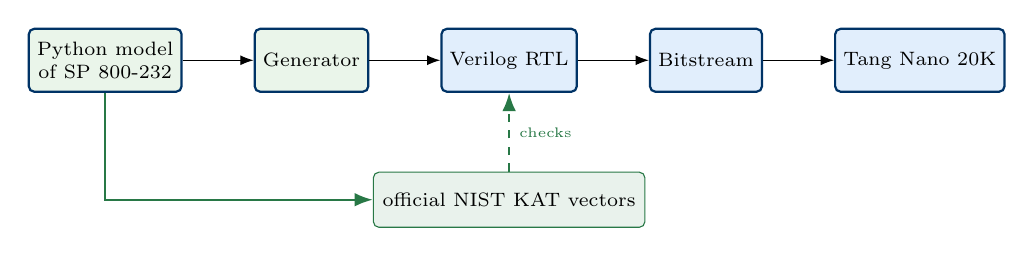
\begin{tikzpicture}[
  >=Latex, node distance=6mm and 9mm,
  b/.style={draw=docblue, thick, rounded corners=2pt, align=center,
            minimum height=8mm, font=\scriptsize, inner sep=3pt},
  sw/.style={b, fill=swfill}, hw/.style={b, fill=hwfill}]
\node[sw] (m) {Python model\\\scriptsize of SP 800-232};
\node[sw, right=of m] (g) {Generator};
\node[hw, right=of g] (r) {Verilog RTL};
\node[hw, right=of r] (b) {Bitstream};
\node[hw, right=of b] (f) {Tang Nano 20K};
\draw[->](m)--(g);\draw[->](g)--(r);\draw[->](r)--(b);\draw[->](b)--(f);
\node[draw=okgreen, fill=okgreen!10, rounded corners=2pt, below=10mm of r,
      font=\scriptsize, minimum height=7mm] (kat) {official NIST KAT vectors};
\draw[->, okgreen, thick] (m.south) |- (kat.west);
\draw[->, okgreen, thick, dashed] (kat.north) -- (r.south) node[midway, right, font=\tiny, okgreen] {checks};
\end{tikzpicture}

\vspace{4mm}
\begin{columns}[T]
\begin{column}{0.5\textwidth}
\begin{block}{One source of truth}
\small The model is both the \textbf{source} of the hardware and the \textbf{oracle}
that checks it. The RTL and the test vectors descend from the same validated
definition.
\end{block}
\end{column}
\begin{column}{0.5\textwidth}
\begin{block}{The consequence, borne out}
\small Every bug that reached the board was an \textbf{integration} bug --- a bus
handshake, a protocol order. \alert{Not one was a cryptographic bug.}
\end{block}
\end{column}
\end{columns}
\end{frame}

\begin{frame}{The accelerator: five layers, each checked alone}
\centering
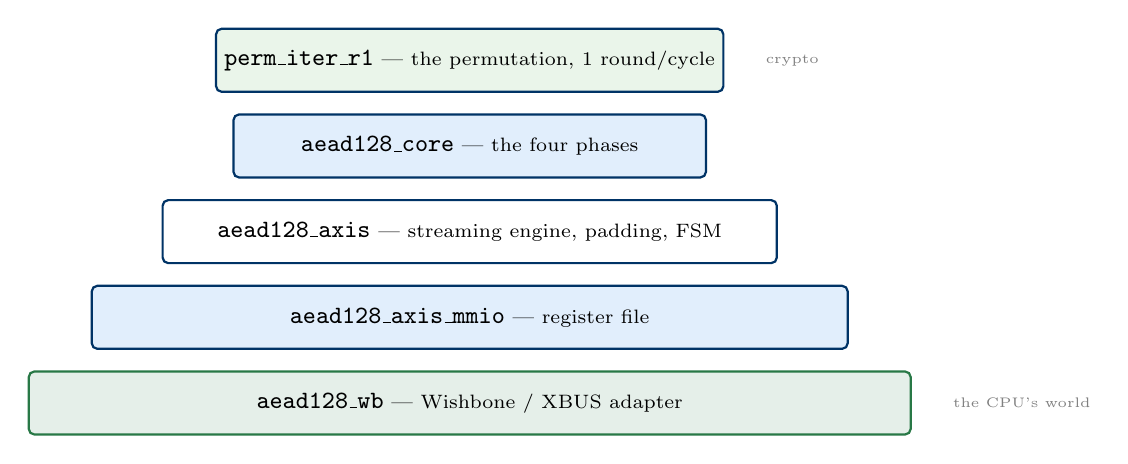
\begin{tikzpicture}[
  >=Latex, node distance=2.6mm,
  L/.style={draw=docblue, thick, rounded corners=2pt, align=center,
            minimum height=8mm, font=\scriptsize, inner sep=3pt}]
\node[L, fill=swfill, minimum width=42mm] (p) {\code{perm\_iter\_r1} --- the permutation, 1 round/cycle};
\node[L, fill=hwfill, minimum width=60mm, below=of p] (c) {\code{aead128\_core} --- the four phases};
\node[L, fill=white, minimum width=78mm, below=of c] (a) {\code{aead128\_axis} --- streaming engine, padding, FSM};
\node[L, fill=hwfill, minimum width=96mm, below=of a] (m) {\code{aead128\_axis\_mmio} --- register file};
\node[L, fill=okgreen!12, draw=okgreen, minimum width=112mm, below=of m] (w) {\code{aead128\_wb} --- Wishbone / XBUS adapter};
\node[right=4mm of p, font=\tiny, gray] {crypto};
\node[right=4mm of w, font=\tiny, gray] {the CPU's world};
\end{tikzpicture}

\vspace{3mm}
{\small One job per layer, each replayed against the model in isolation --- so a
failure names its own layer. The bottom layer is where all the trouble was.}
\end{frame}

\begin{frame}{Integration: a peripheral, not a custom instruction}
\begin{columns}[T]
\begin{column}{0.47\textwidth}
\begin{itemize}\small
\item CPU: NEORV32, \code{rv32i}, 27\,MHz --- completely \textbf{stock}.
\item The accelerator hangs off the \textbf{external} bus (XBUS) at
      \code{0x9000\_0000}: \alert{no CPU pipeline changes}, no custom instructions.
\item The driver hides every register behind \code{encrypt()} / \code{decrypt()}.
\end{itemize}
\vspace{1mm}
{\small\color{docblue}\textbf{Why not a custom instruction?}}\\
{\footnotesize Tighter coupling would cut data movement --- a real advantage, and
where the future work points. But it welds the design to one pipeline. On a
standard bus the interface is public, portable and testable.}
\end{column}
\begin{column}{0.53\textwidth}
\vspace{-1mm}
\centering
\scalebox{0.86}{%
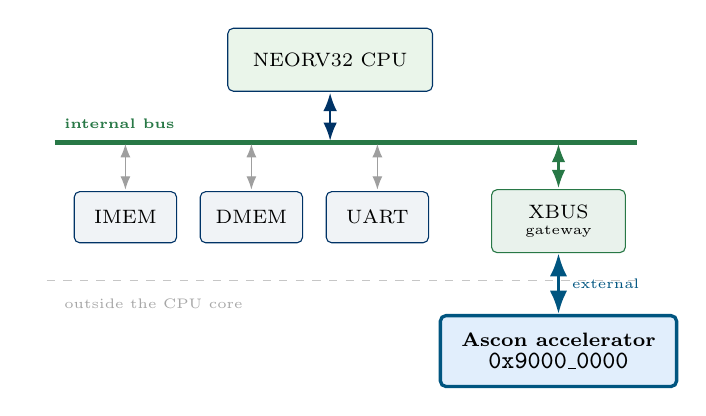
\begin{tikzpicture}[font=\scriptsize, >=Latex,
  blk/.style={draw=docblue, rounded corners=2pt, minimum width=13mm,
              minimum height=6.5mm, fill=docblue!6, inner sep=2pt},
  acc/.style={draw=doclblue, very thick, rounded corners=2pt, fill=hwfill,
              minimum width=30mm, minimum height=9mm, align=center}]

% --- CPU ---
\node[blk, minimum width=26mm, minimum height=8mm, fill=swfill] (cpu) at (0,3.15) {NEORV32 CPU};

% --- internal bus bar ---
\draw[okgreen, line width=1.6pt] (-3.5,2.1) -- (3.9,2.1);
\node[font=\tiny\bfseries, okgreen, above right] at (-3.5,2.15) {internal bus};
\draw[<->, docblue, thick] (0,2.73) -- (0,2.12);

% --- internal peripherals, each dropping straight from the bar ---
\node[blk] (imem) at (-2.6,1.15) {IMEM};
\node[blk] (dmem) at (-1.0,1.15) {DMEM};
\node[blk] (uart) at (0.6,1.15) {UART};
\foreach \x in {-2.6,-1.0,0.6}{ \draw[<->, gray!75] (\x,2.08) -- (\x,1.5); }

% --- XBUS gateway ---
\node[blk, minimum width=17mm, minimum height=8mm, fill=okgreen!10, draw=okgreen] (gw) at (2.9,1.1)
  {\shortstack{XBUS\\\tiny gateway}};
\draw[<->, okgreen, thick] (2.9,2.08) -- (2.9,1.52);

% --- the accelerator, on the external side ---
\node[acc] (acc) at (2.9,-0.55) {\textbf{Ascon accelerator}\\\code{0x9000\_0000}};
\draw[<->, doclblue, very thick] (gw.south) -- (acc.north)
  node[midway, right=1pt, font=\tiny, doclblue] {external};

% --- boundary ---
\draw[gray!45, dashed] (-3.6,0.35) -- (3.9,0.35);
\node[font=\tiny, gray!70, left] at (-3.6,0.35) {};
\node[font=\tiny, gray!70, align=left, anchor=west] at (-3.5,0.05) {outside the CPU core};
\end{tikzpicture}}
\end{column}
\end{columns}
\end{frame}

\begin{frame}{A fully-open, reproducible toolchain}
\centering
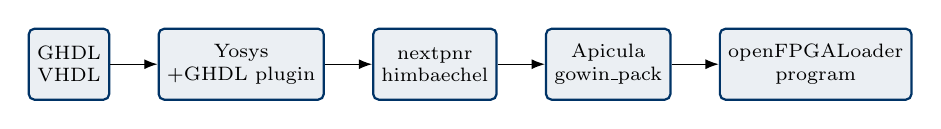
\begin{tikzpicture}[
  >=Latex, node distance=6mm, font=\scriptsize,
  t/.style={draw=docblue, thick, rounded corners=2pt, fill=docblue!8,
            align=center, minimum height=9mm, inner sep=3pt}]
\node[t](a){GHDL\\\scriptsize VHDL};
\node[t,right=of a](b){Yosys\\\scriptsize +GHDL plugin};
\node[t,right=of b](c){nextpnr\\\scriptsize himbaechel};
\node[t,right=of c](d){Apicula\\\scriptsize gowin\_pack};
\node[t,right=of d](e){openFPGALoader\\\scriptsize program};
\draw[->](a)--(b);\draw[->](b)--(c);\draw[->](c)--(d);\draw[->](d)--(e);
\end{tikzpicture}

\vspace{6mm}
\begin{block}{No vendor EDA at any step}
\small Every stage from VHDL/Verilog to a programmed FPGA is open source, and the
exact versions are pinned by a Nix flake. \code{nix flake check} runs the whole
test suite from a clean checkout.
\end{block}
\end{frame}

% ============================================================
\section{Verification}

\begin{frame}{Four layers of verification}
\small
\begin{center}
\begin{tabular}{cll}
\toprule
\textbf{Layer} & \textbf{What is checked} & \textbf{Against}\\
\midrule
1 & The Python model & the official NIST Known-Answer Tests\\
2 & Every generated RTL module & the model (25 vectors per module)\\
3 & The C driver & an emulated peripheral\\
4 & End-to-end co-simulation & a NEORV32-faithful XBUS master\\
\bottomrule
\end{tabular}
\end{center}
\vspace{3mm}
\begin{block}{119 automated tests}
\small Run from a clean checkout; reproduced by \code{nix flake check}. Layer~4
replays the driver's real register order through the bus adapter with NEORV32's
exact pulsed-strobe timing --- it exists \emph{because} of the bug on the next
slide but one.
\end{block}
\end{frame}

\begin{frame}{From ``simulation passes'' to ``correct on silicon''}
\small Eight real bugs --- each diagnosed from the board's own evidence, not guesswork:
\begin{columns}[T]
\begin{column}{0.5\textwidth}
\begin{enumerate}
\item Read-only build environment
\item Toolchain name mismatch
\item Float-ABI (double vs.\ soft) mismatch
\item \textbf{Stack past end of RAM} $\to$ silent trap
\end{enumerate}
\end{column}
\begin{column}{0.5\textwidth}
\begin{enumerate}\setcounter{enumi}{4}
\item Flaky USB debugger / shifting ports
\item \alert{\textbf{XBUS bus handshake}}
\item FPGA fit (drop the M extension)
\item \alert{\textbf{START-first protocol order}}
\end{enumerate}
\end{column}
\end{columns}
\vspace{2mm}
\begin{block}{Evidence, not guessing}
\small A processor panic with a precise fault address (\code{0x9000\,0000}, then
\code{0x9000\,0044}) named exactly which register --- and which mechanism --- had
failed.
\end{block}
\end{frame}

\begin{frame}{The key hardware bug: the bus handshake}
\begin{columns}[T]
\begin{column}{0.54\textwidth}
\small
\textbf{NEORV32's XBUS:}
\begin{itemize}
\item pulses the strobe for \emph{one cycle}
\item samples the acknowledge only in the \emph{next} cycle
\end{itemize}
\vspace{2mm}
\textbf{My first adapter:} acknowledged \emph{during} the strobe --- the one cycle
the CPU was not looking.
\vspace{2mm}
$\Rightarrow$ no ack seen $\to$ bus timeout $\to$ \alert{access fault at
\code{0x9000\_0000}}.
\vspace{2mm}
\textbf{Fix:} a handshake FSM that latches the strobe, holds the access until the
peripheral is ready, and acks in the cycle the CPU samples.
\end{column}
\begin{column}{0.46\textwidth}
\centering
\scalebox{0.76}{%
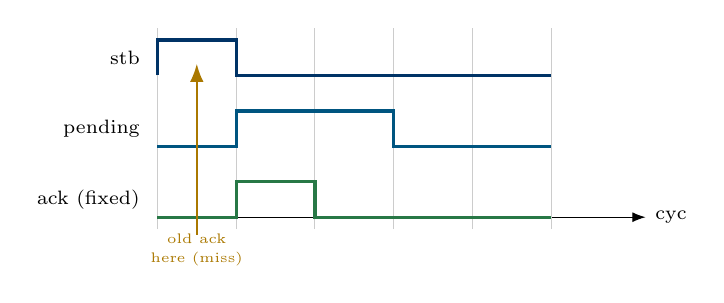
\begin{tikzpicture}[font=\scriptsize, >=Latex, yscale=0.75]
\draw[->](0,0)--(6.2,0) node[right]{cyc};
\foreach \x in {0,1,...,5}\draw[gray!40](\x,-0.2)--(\x,3.2);
\node[left] at (-0.1,2.7){stb};
\draw[docblue,very thick](0,2.4)--(0,3.0)--(1,3.0)--(1,2.4)--(5,2.4);
\node[left] at (-0.1,1.5){pending};
\draw[doclblue,very thick](0,1.2)--(1,1.2)--(1,1.8)--(3,1.8)--(3,1.2)--(5,1.2);
\node[left] at (-0.1,0.3){ack (fixed)};
\draw[okgreen,very thick](0,0)--(1,0)--(1,0.6)--(2,0.6)--(2,0)--(5,0);
\node[warnamber, font=\tiny] at (0.5,-0.55){\shortstack{old ack\\here (miss)}};
\draw[warnamber,->,thick](0.5,-0.3)--(0.5,2.6);
\end{tikzpicture}}
\vspace{2mm}
{\scriptsize Against a naive testbench this passes. Against the real CPU it fails
every time --- so Layer~4 now models the CPU exactly.}
\end{column}
\end{columns}
\end{frame}

% ============================================================
\section{Results}

\begin{frame}{Correct on hardware, and 18--57$\times$ faster}
\small All 8 cases correct on the board (\code{enc\_ok}, \code{dec\_ok},
\code{tag\_valid}). Cycles at 27\,MHz:
\begin{center}
\renewcommand{\arraystretch}{1.05}
\begin{tabular}{lccrrc}
\toprule
\textbf{Case} & \textbf{AD} & \textbf{PT} & \textbf{SW} & \textbf{HW} & \textbf{Speed-up}\\
\midrule
\code{empty}     & 0  & 0  & 38\,866 & 684   & \textbf{56.8}$\times$\\
\code{ad8}       & 8  & 0  & 50\,205 & 1\,335 & 37.6$\times$\\
\code{pt8}       & 0  & 8  & 39\,458 & 1\,239 & 31.8$\times$\\
\code{ad8\_pt8}  & 8  & 8  & 50\,797 & 1\,890 & 26.9$\times$\\
\code{pt16}      & 0  & 16 & 52\,156 & 2\,007 & 26.0$\times$\\
\code{pt24}      & 0  & 24 & 52\,748 & 2\,763 & 19.1$\times$\\
\code{pt32}      & 0  & 32 & 65\,447 & 3\,531 & 18.5$\times$\\
\code{ad16\_pt32}& 16 & 32 & 86\,984 & 4\,948 & 17.6$\times$\\
\bottomrule
\end{tabular}
\end{center}
{\small Cases probe the block structure: empty, AD only, PT only, both, and
partial vs.\ full 16-byte rate blocks.}
\end{frame}

\begin{frame}{Results, visualised}
\begin{columns}[c]
\begin{column}{0.52\textwidth}
\centering
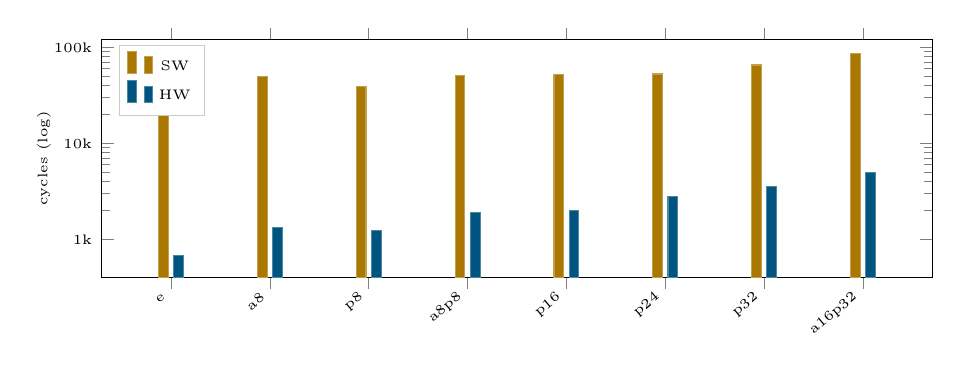
\begin{tikzpicture}
\begin{axis}[
  width=\linewidth, height=4.6cm, ybar, bar width=3.5pt,
  ymode=log, log origin=infty, ymin=400, ymax=120000,
  ylabel={\tiny cycles (log)}, ylabel style={yshift=-2mm},
  symbolic x coords={e,a8,p8,a8p8,p16,p24,p32,a16p32},
  xtick=data, x tick label style={rotate=40,anchor=east,font=\tiny},
  ytick={1000,10000,100000}, yticklabels={1k,10k,100k},
  tick label style={font=\tiny},
  legend style={at={(0.02,0.98)},anchor=north west,font=\tiny,draw=gray!40},
  enlarge x limits=0.1]
\addplot[fill=barsw,draw=barsw!70] coordinates{(e,38866)(a8,50205)(p8,39458)(a8p8,50797)(p16,52156)(p24,52748)(p32,65447)(a16p32,86984)};
\addplot[fill=barhw,draw=barhw!70] coordinates{(e,684)(a8,1335)(p8,1239)(a8p8,1890)(p16,2007)(p24,2763)(p32,3531)(a16p32,4948)};
\legend{SW,HW}
\end{axis}
\end{tikzpicture}
{\tiny cycles: software vs.\ hardware}
\end{column}
\begin{column}{0.48\textwidth}
\centering
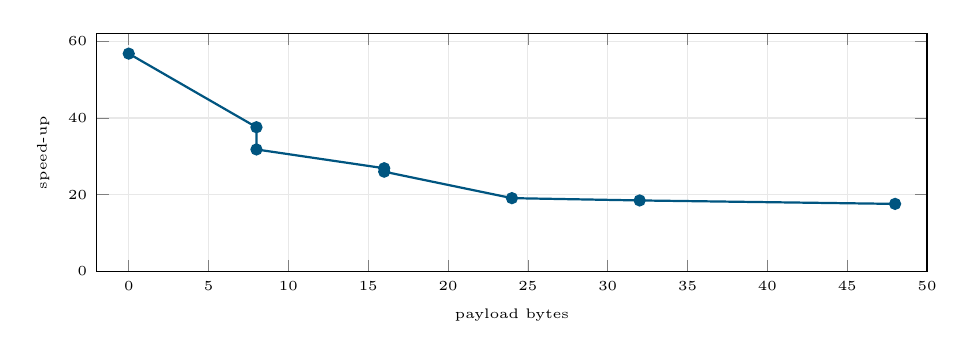
\begin{tikzpicture}
\begin{axis}[
  width=\linewidth, height=4.6cm,
  ylabel={\tiny speed-up}, xlabel={\tiny payload bytes},
  ymin=0, ymax=62, xmin=-2, xmax=50,
  grid=both, grid style={gray!18},
  tick label style={font=\tiny}, mark size=1.8pt]
\addplot[color=barhw,thick,mark=*] coordinates{(0,56.8)(8,37.6)(8,31.8)(16,26.9)(16,26.0)(24,19.1)(32,18.5)(48,17.6)};
\end{axis}
\end{tikzpicture}
{\tiny speed-up falls as payload grows}
\end{column}
\end{columns}
\vspace{2mm}
{\small Larger payloads $\Rightarrow$ more word-at-a-time movement over MMIO
$\Rightarrow$ lower speed-up. \alert{The crypto itself is a handful of cycles.}}
\end{frame}

\begin{frame}{Where the time actually goes}
\small Simulating the AEAD core \emph{alone} --- same vectors, data already
present --- separates \emph{crypto} from \emph{waiting for data}:
\begin{center}
{\footnotesize\setlength{\tabcolsep}{5pt}
\begin{tabular}{lrrrr}
\toprule
\textbf{Case} & \textbf{HW busy} & \textbf{Crypto} & \textbf{Waiting on I/O} & \textbf{Crypto \%}\\
\midrule
\code{empty}     & 684   & 36 & 648   & 5.3\,\%\\
\code{pt16}      & 2\,007 & 48 & 1\,959 & 2.4\,\%\\
\code{pt32}      & 3\,531 & 60 & 3\,471 & 1.7\,\%\\
\code{ad16\_pt32}& 4\,948 & 83 & 4\,865 & \textbf{1.7\,\%}\\
\midrule
\textbf{all 8 cases} & \textbf{18\,397} & \textbf{405} & \textbf{17\,992} & \textbf{2.2\,\%}\\
\bottomrule
\end{tabular}}
\end{center}
\vspace{1mm}
\begin{block}{The bottleneck is the interface, and it is not close}
\small
\begin{itemize}\small
\item Make the permutation \textbf{8$\times$ faster} (the 8-rounds/cycle core I
      already have): 17.6$\times$ $\rightarrow$ 17.8$\times$. \alert{+0.2$\times$.}
\item Remove the data-movement cost entirely (an upper bound, not a design):
      17.6$\times$ $\rightarrow$ \textbf{$\sim$1050$\times$}.
\end{itemize}
\end{block}
\end{frame}

\begin{frame}{So I rebuilt the data plane --- and measured it on silicon}
\begin{columns}[T]
\begin{column}{0.44\textwidth}
{\small The engine was \emph{already} AXI4-Stream native. One line in the MMIO
wrapper was the entire bottleneck:}
\vspace{1mm}

{\scriptsize\code{wire s\_tvalid = din\_ctl\_wr;}}

{\footnotesize A streaming datapath, clocked by a \textbf{CPU store}.}
\vspace{1.5mm}

{\small\color{docblue}\textbf{The replacement}}\\
{\footnotesize NEORV32's \textbf{SLINK} is AXI4-Stream at 32 bits --- an exact
match --- and its \textbf{DMA} takes a constant destination address:}

{\scriptsize DMEM $\rightarrow$ DMA $\rightarrow$ SLINK $\rightarrow$
\textbf{Ascon} $\rightarrow$ SLINK $\rightarrow$ DMA $\rightarrow$ DMEM}
\vspace{1mm}

{\footnotesize The CPU writes key, nonce, lengths and START --- then touches
\textbf{no payload byte at all}.}
\end{column}
\begin{column}{0.56\textwidth}
\vspace{-2mm}
\centering
{\scriptsize\setlength{\tabcolsep}{4pt}\renewcommand{\arraystretch}{1.05}
\begin{tabular}{lrrrr}
\toprule
& \multicolumn{2}{c}{\textbf{busy cycles}} & \multicolumn{2}{c}{\textbf{vs software}}\\
\cmidrule(lr){2-3}\cmidrule(lr){4-5}
\textbf{Case} & MMIO & \textbf{SLINK} & MMIO & \textbf{SLINK}\\
\midrule
empty      &   684 &  \textbf{41} & 56.8$\times$ & \textbf{948$\times$}\\
ad8        & 1\,335 & \textbf{296} & 37.6$\times$ & \textbf{170$\times$}\\
pt8        & 1\,239 & \textbf{286} & 31.8$\times$ & \textbf{138$\times$}\\
pt16       & 2\,007 & \textbf{336} & 26.0$\times$ & \textbf{155$\times$}\\
pt32       & 3\,531 & \textbf{432} & 18.5$\times$ & \textbf{152$\times$}\\
\rowcolor{hwfill}
ad16\_pt32 & 4\,948 & \textbf{535} & 17.6$\times$ & \textbf{163$\times$}\\
\midrule
\textbf{total} & \textbf{18\,397} & \textbf{2\,639} & \multicolumn{2}{c}{\textbf{7.0$\times$ fewer}}\\
\bottomrule
\end{tabular}}
\vspace{2mm}

{\footnotesize \textbf{8/8 correct on the board.} Same vectors, same counter.
Crypto share: \textbf{2.2\% $\rightarrow$ 15.3\%}.}
\end{column}
\end{columns}
\end{frame}

\begin{frame}{The new bottleneck --- measured the same way}
{\small Simulation predicted 118 cycles for \code{ad16\_pt32}; silicon gave 535.
That gap is not noise. It is the DMA, and it fits a straight line.}
\vspace{1mm}
\begin{columns}[c]
\begin{column}{0.48\textwidth}
\centering
{\scriptsize\setlength{\tabcolsep}{5pt}\renewcommand{\arraystretch}{1.08}
\begin{tabular}{lrrrr}
\toprule
\textbf{Case} & \textbf{words} & \textbf{sim} & \textbf{silicon} & \textbf{gap}\\
\midrule
\rowcolor{okgreen!12}
empty      &  0 &  41 &  41 & \textbf{0}\\
ad8        &  2 &  55 & 296 & 241\\
ad8\_pt8   &  4 &  60 & 333 & 273\\
pt24       &  6 &  69 & 380 & 311\\
pt32       &  8 &  87 & 432 & 345\\
ad16\_pt32 & 12 & 118 & 535 & 417\\
\bottomrule
\end{tabular}}
\end{column}
\begin{column}{0.52\textwidth}
\begin{center}
\fbox{\parbox{0.92\textwidth}{\centering\small
$\text{overhead} = \mathbf{204} + \mathbf{17.7} \times \text{words}$\\[1mm]
{\footnotesize fits every case to within \textbf{2 cycles}}}}
\end{center}
\vspace{1mm}
\begin{itemize}\footnotesize
\item \textbf{204 cycles} --- programming and starting one DMA descriptor.
\item \textbf{17.7 cycles/word} --- NEORV32's DMA is a read-then-write engine,
      not a burst master.
\item \code{empty} sends no words, so it has \textbf{zero} overhead --- and lands
      exactly on the simulated 41.
\end{itemize}
\end{column}
\end{columns}
\vspace{1mm}
{\small\color{docblue}\textbf{So: the stream datapath is precisely as designed. The entire shortfall is the data mover.}}\\
{\footnotesize Which is, once again, a measurement rather than a guess --- and it
names the next piece of work: a burst-capable master, not a faster permutation.}
\end{frame}

\begin{frame}{Faster than \emph{what}? --- being precise}
\begin{block}{The comparison}
\small \textbf{Software} = \code{rdcycle} around a reference C Ascon-AEAD128 on the
same \code{rv32i} core. \quad
\textbf{Hardware} = the accelerator's busy-cycle counter, same 27\,MHz.
\end{block}
\vspace{1mm}
\alert{Caveats, stated plainly:}
\begin{itemize}\small
\item The software is a \emph{reference}, not hand-optimised --- an optimised
      version would narrow the gap (hardware still wins).
\item The hardware counter excludes register setup and readback; the full
      end-to-end wall-clock number is lower, especially for \code{empty}.
\item The $\sim$18$\times$ on real payloads is much closer to end-to-end than the
      $\sim$57$\times$ on the empty case.
\end{itemize}
\vspace{1mm}
{\small Fair phrasing: \textbf{the hardware engine vs.\ reference software on the
same SoC} --- same platform, same clock, same counter.}
\end{frame}

% ============================================================
\section{Conclusions}

\begin{frame}{Limitations \& future work}
\begin{columns}[T]
\begin{column}{0.5\textwidth}
{\small\color{warnamber}\textbf{Limitations --- stated, not hidden}}
\begin{itemize}\footnotesize
\item \textbf{Bounded payload}: 32\,B AD + 32\,B message. Chosen so the length
      handling could be verified exhaustively.
\item \textbf{No side-channel hardening.} No masking, no fault countermeasures,
      no characterisation. The tag compare is constant-time by construction; that
      is one channel, not a claim.
\item \textbf{Key registers are readable.} Mirrored from the reference map and
      never hardened --- a defect for a product.
\item \textbf{Hash/XOF exist in the model only}, not on the board.
\item \textbf{86.5\% LUT utilisation} forced \code{RISCV\_ISA\_M} off.
\end{itemize}
\end{column}
\begin{column}{0.5\textwidth}
{\small\color{okgreen}\textbf{Done since the measurement}}
\begin{itemize}\footnotesize
\item \textbf{The data plane is rebuilt and on silicon}: SLINK + DMA,
      \textbf{17.6$\times \rightarrow$ 163$\times$}, 8/8 correct.
\end{itemize}
\vspace{1mm}
{\small\color{docblue}\textbf{Next --- and now measured, not guessed}}
\begin{itemize}\footnotesize
\item \textbf{A burst-capable master.} The DMA costs $204 + 17.7 \times
      \text{words}$; that, not the permutation, is the remaining 85\%.
\item \textbf{Then} the faster permutation earns its area --- at 15\% crypto it
      finally moves the number.
\item Arbitrary-length streaming; hash/XOF on hardware; a hardened key path.
\end{itemize}
\end{column}
\end{columns}
\end{frame}

\begin{frame}{Conclusion}
\begin{columns}[T]
\begin{column}{0.5\textwidth}
{\small\color{docblue}\textbf{What was achieved}}
\begin{itemize}\footnotesize
\item A \textbf{model-driven} Ascon-AEAD128 accelerator: one typed Python model,
      anchored to the official NIST vectors, that \emph{generates} the RTL
      \emph{and} verifies it.
\item \textbf{Seven permutation architectures} from that one model, all verified
      --- a \textbf{120$\times$} latency span.
\item \textbf{Silicon}, not simulation: a stock NEORV32 SoC on a Tang Nano 20K,
      8/8 correct, entirely open toolchain.
\item \textbf{119 automated tests}, reproducible with \code{nix flake check}.
\end{itemize}
\end{column}
\begin{column}{0.5\textwidth}
{\small\color{docblue}\textbf{What I would want you to take away}}
\vspace{1mm}

{\footnotesize I measured before I optimised. The measurement said the crypto was
\textbf{2.2\%} of the time and the interface was \textbf{97.8\%} --- so a faster
permutation was worth $+0.2\times$ and was not the answer.}
\vspace{1mm}

{\footnotesize So I rebuilt the data plane instead. On the board:
\textbf{17.6$\times \rightarrow$ 163$\times$}, and the crypto share rose from
2.2\% to 15.3\%.}
\vspace{1mm}

{\footnotesize And the new bottleneck is measured too:
$204 + 17.7 \times \text{words}$ of DMA. Not a guess --- a straight line through
eight silicon data points.}
\vspace{2mm}

\begin{center}
\fbox{\parbox{0.92\textwidth}{\centering\footnotesize
\textbf{Measure. Fix the thing the measurement names.}\\
\textbf{Measure again.}}}
\end{center}
\end{column}
\end{columns}
\end{frame}

\end{document}
